\documentclass{article}
\usepackage{graphicx} % Required for inserting images
\usepackage{varwidth}
\usepackage{xcolor}
\usepackage{listings}


\definecolor{codegreen}{rgb}{0,0.6,0}
\definecolor{codegray}{rgb}{0.5,0.5,0.5}
\definecolor{codepurple}{rgb}{0.58,0,0.82}
\definecolor{backcolour}{rgb}{0.95,0.95,0.92}

\lstdefinestyle{CStyle}{
	language=C++,
	backgroundcolor=\color{backcolour},   
	commentstyle=\color{codegreen},
	keywordstyle=\color{magenta},
	numberstyle=\tiny\color{codegray},
	stringstyle=\color{codepurple},
	basicstyle=\ttfamily\footnotesize,
	breakatwhitespace=false,         
	breaklines=true,                 
	keepspaces=true,                 
	numbers=left,       
	numbersep=5pt,                  
	showspaces=false,                
	showstringspaces=false,
	showtabs=false,                  
	tabsize=2,
}
\lstset{style=CStyle}

\title{Lab 7 Report \\ \large EEL4742C - 00446}
\author{Yousef Awad}
\date{September 2025}
\setcounter{secnumdepth}{0}

\begin{document}

\maketitle
\tableofcontents
\newpage

\section{Introduction}
In this lab, we learned how to use the I2C module on the MSP430 as well as what I2C is generally, via programming the I2C link that connects the board to the booster pack that we put on it.

\section{7.1 I2C Transmission}
Now, in this section we are told to answer some questions!! YIPPEEEE!!!! So let's get into it, shall we? The sensor can specifically have the following 4 address, via editing the ADDR pin on the light sensor. They are:
\begin{itemize}
  \item 0x44: GND (Ground)
  \item 0x45: VDD (Voltage)
  \item 0x46: SDA (Serial Data)
  \item 0x47: SCL (Serial Clock)
\end{itemize}
Now, since the default address (first address) of the light sensor is 0x44, it also means that ADDR is 0x44 and therefore is connected to the ground. Now, for the I2C lines, they are using a pull-up resistor of $10k\Omega$ (screenshot of the schematic being right below this very paragraph). And, when using the code below, we see a manufacturer ID of TI, and a device ID of 0x3001. 
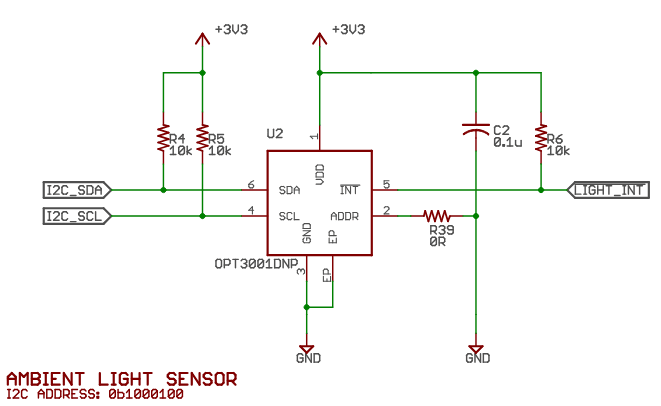
\includegraphics[width=1\textwidth]{pictures/image.png}
\pagebreak
\lstinputlisting{7_1.c}
\pagebreak

\section{7.2 Reading Measurements from the Light Sensor}
Now, for this part of the lab, we are told to answer MORE questions (crazy, I know). THEREFORE, to make you're life easier, I'm going to... guess what... ANSWER THEM!!!!!! The address of the config register on the sensor is 0x01. And the value that I used, in HEX (because that's how you want it) was 0x7614 or into the bit fields to be 0111 0110 0000 0100. And, thankfully, the sensor readings seem very sensible (get it, sensor.... sensible??? I'm not the only one laughing, right???), as well as consistent.
\lstinputlisting{7_2.c}
\pagebreak

\section{Student Q\&A}
\subsection{1}
\textbf{Given:} \textit{The light sensor has an address pin that allows customizing the I2C address. How many addresses are possible? What are they and how are they configured? Look in the sensor’s data sheet.}
\newline
The light sensor has 4 addresses that are possible. They are:
\begin{itemize}
  \item 0x44: GND (Ground)
  \item 0x45: VDD (Voltage)
  \item 0x46: SDA (Serial Data)
  \item 0x47: SCL (Serial Clock)
\end{itemize}

\subsection{2}
\textbf{Given:} \textit{According to the light sensor’s data sheet, what should be the value of the pull-up resistors on the I2C wires? Did the BoosterPack use the same values?}
\newline
The value of the pull-up resistor is $10k\Omega$ in the BoosterPack, and is, as well, the same value that is recommended by the light sensor's data sheet.

\subsection{3}
\textbf{Given:} \textit{What I2C clock frequency do each of the eUSCI module and the sensor support?}
\newline
The MSP430 supports only standard and fast mode, or 100KHz and 400KHz, only. However, the light sensor supports all 3 modes of I2C, being standard, fast, and high-speed, or 100KHz, 400KHz, and 2.6MHz.

\end{document}
